\documentclass[jou]{apa6}

\usepackage[american]{babel}

\usepackage{csquotes}
\usepackage[style=apa,sortcites=true,sorting=nyt,backend=biber]{biblatex}
\DeclareLanguageMapping{american}{american-apa}
\addbibresource{bibliography.bib}


%%%%%%%%%%%%%%%%%%%%%%%%%%%%%%%%%%%%%%%%
%% Discrete Structures
%% The start of RBS stuff
%%%%%%%%%%%%%%%%%%%%%%%%%%%%%%%%%%%%%%%%

% Working internal and external links in PDF
\usepackage{hyperref}
% Extra math symbols in LaTeX
\usepackage{amsmath}
\usepackage{gensymb}
\usepackage{amssymb}
% Enumerations with (a), (b), etc.
\usepackage{enumerate}

\let\OLDitemize\itemize
\renewcommand\itemize{\OLDitemize\addtolength{\itemsep}{-6pt}}

\usepackage{etoolbox}
\makeatletter
\preto{\@verbatim}{\topsep=3pt \partopsep=3pt }
\makeatother

% These sizes redefine APA for A4 paper size
\oddsidemargin 0.0in
\evensidemargin 0.0in
\textwidth 6.27in
\headheight 1.0in
\topmargin -24pt
\headheight 12pt
\headsep 12pt
\textheight 9.19in



\title{Sample Quiz 8}
\author{Discrete Structures, Spring 2020}
\affiliation{RBS}

\leftheader{Discrete Sample Quiz 8}

\abstract{%
}

%\keywords{}

\setlength\parindent{0pt}

\begin{document}

%\thispagestyle{empty}

\twocolumn
\section{Worksheet 12: Trees}

{\bf Question 1.} Count the objects:\\
{\bf (A)} If $T$ is a tree with $999$ vertices, then $T$ has $\ldots$ edges.\\
{\bf (B)} There are $\ldots$ non-isomorphic trees with four vertices.\\
{\bf (C)} There are $\ldots$ non-isomorphic rooted trees with four vertices (isomorphism 
for rooted trees can change map any node to any other; but it should map root to root).\\
{\bf (D)} There are $\ldots$ full binary trees with six vertices.\\
{\bf (E)} The cycle graph $C_7$ has $\ldots$ spanning trees.\\
{\bf (F)} If $T$ is a binary tree with 100 vertices, its minimum height is $\ldots$.\\
{\bf (G)} If $T$ is a full binary tree with $101$ vertices, its minimum height is $\ldots$.\\
{\bf (H)} If $T$ is a full binary tree with $101$ vertices, its maximum height is $\ldots$.\\
{\bf (I)} If $T$ is a full binary tree with $50$ leaves, its minimum height is $\ldots$.\\
{\bf (J)} Every full binary tree with $61$ vertices has $\ldots$ leaves.\\
{\bf (K)} Every full binary tree with $50$ leaves has $\ldots$ vertices.\\
{\bf (L)} Every 3-ary tree with 13 vertices has $\ldots$ leaves.

\vspace{10pt}
{\bf Question 2.} Find, if a statement is true or false:\\
{\bf (A)} If T is a tree with 17 vertices, then there is a simple path in T of length 17.\\
{\bf (B)} Every tree is bipartite.\\
{\bf (C)} There is a tree with degrees $3, 2, 2, 2, 1, 1, 1, 1, 1$.\\
{\bf (D)} There is a tree with degrees $3, 3, 2, 2, 1, 1, 1, 1$.\\
{\bf (E)} If two trees have the same number of vertices and the same degrees, then the two trees are isomorphic.\\
{\bf (F)} If $T$ is a tree with $50$ vertices, the largest degree that any vertex can have is $49$.\\
{\bf (G)} In a binary tree with $16$ vertices, there must be a path of length $4$.\\
{\bf (H)} If $T$ is a rooted binary tree of height $5$, then $T$ has at most $25$ leaves.


\vspace{10pt}
{\bf Question 3.}\\
Suppose you have $50$ coins, one of which is counterfeit 
(either heavier or lighter than the others). You use a
balance scale to find the bad coin. Prove that $4$ weighings 
are not enough to guarantee that you find the
bad coin and determine whether 
it is heavier or lighter than the other coins.


\vspace{10pt}
{\bf Question 4.}\\
Suppose you have $5$ coins, one of which is counterfeit 
(either heavier or lighter than the other four). You use
a pan balance scale to find the bad coin and determine 
whether it is heavier or lighter.\\
{\bf (A)} Prove that $2$ weighings are not enough to guarantee 
that you find the bad coin and determine whether it
is heavier or lighter.\\
{\bf (B)}  Draw a decision tree for weighing the coins to determine 
the bad coin (and whether it is heavier or lighter)
in the minimum number of weighings.


\vspace{10pt}
{\bf Question 5.}\\
Suppose you have $5$ coins, one of which is heavier than the other four. 
Draw the decision tree for using a
balance scale to find the heavy coin. How many weighings would you need?



\vspace{10pt}
{\bf Question 6.} 
\begin{figure}[!htb]
\center{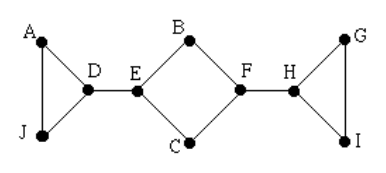
\includegraphics[width=2.5in]{quiz-sample-12/quiz12-graph.png}}
\caption{\label{fig:quiz12-graph} Graph for DFS and BFS traversal.}
\end{figure}


{\bf (A)} Using alphabetical ordering, find a spanning tree for the graph on Figure~\ref{fig:quiz12-graph} by using a depth-first search.\\
{\bf (B)} Using alphabetical ordering, find a spanning tree for this graph by using a breadth-first search.\\
{\bf (C)} Using the ordering $C, D, E, F, G, H, I, J, A, B$, find a spanning tree for this graph by using a depth-first search.\\
{\bf (D)} Using the ordering $C, D, E, F, G, H, I, J, A, B$, find a spanning tree for this graph by using a breadth-first search.\\
{\bf (E)} Using reverse alphabetical ordering, find a spanning tree for the graph by using a depth-first search.\\
{\bf (F)} Using reverse alphabetical ordering, find a spanning tree for the graph by using a breadth-first search.






\vspace{10pt}
{\bf Question 7.}\\
Write the compound proposition $(\neg p) \rightarrow (q \vee (r \wedge \neg s))$ 
as the abstract syntax tree ($\neg$, $\rightarrow$, $\vee$ and $\wedge$ operators
are inner nodes; but $p,q,r,s$ are leaves).\\
List the graph nodes in pre-order, in-order and post-order traversal of this syntax tree.


\vspace{10pt}
{\bf Question 8.}\\
Draw the abstract syntax tree, the preorder and postorder traversal 
of $(8x - y)^5 - 7\sqrt{4z - 3}$.


\vspace{10pt}
{\bf Question 9.} 
The string\\
$p\;r\;q\;\rightarrow\;\neg\;q\;\triangle\;p\;\rightarrow\;\wedge$\\
is postfix notation for a logic expression; however, there is a misprint. The
triangle should be one of these three: $r$, $\vee$, or $\neg$. 
Determine which of these three it must be and explain your
reasoning.


\mbox{}
\newpage
\subsection{Answers}

\vspace{10pt}
{\bf Question 1.} Answer:\\
{\bf (A)} If $T$ is a tree with $999$ vertices, then $T$ has $998$ edges.\\
{\bf (B)} There are $2$ non-isomorphic trees with four vertices.\\
{\bf (C)} There are $4$ non-isomorphic rooted trees with four vertices.\\
{\bf (D)} There are $0$ full binary trees with six vertices.\\
{\bf (E)} The cycle graph $C_7$ has $7$ spanning trees.\\
{\bf (F)} If $T$ is a binary tree with 100 vertices, its minimum height is $6$.\\
{\bf (G)} If $T$ is a full binary tree with $101$ vertices, its minimum height is $6$.\\
{\bf (H)} If $T$ is a full binary tree with $101$ vertices, its maximum height is $50$.\\
{\bf (I)} If $T$ is a full binary tree with $50$ leaves, its minimum height is $6$.\\
{\bf (J)} Every full binary tree with $61$ vertices has $31$ leaves.\\
{\bf (K)} Every full binary tree with $50$ leaves has $99$ vertices.\\
{\bf (L)} Every 3-ary tree with 13 vertices has $9$ leaves.

\vspace{10pt}
{\bf Question 2.} Answer: TBD \\

\vspace{10pt}
{\bf Question 3.} Answer:\\

Four weighings could give at most $3^4 = 81$ outcomes (each time we use scales there are
three possible results). But the problem has $2 \cdot 50$ different situations
(any of the $50$ coins can be different; and it can be either heavier or lighter). 

\vspace{10pt}
{\bf Question 4.} Answer: TBD \\

\vspace{10pt}
{\bf Question 5.} Answer: TBD \\

\vspace{10pt}
{\bf Question 6.} Answer: TBD \\

\vspace{10pt}
{\bf Question 7.} Answer: TBD \\

\vspace{10pt}
{\bf Question 8.} Answer: TBD \\

\vspace{10pt}
{\bf Question 9.} Answer: TBD \\






\end{document}

